\documentclass[a4paper, 12pt, oneside]{scrbook}
\usepackage[hyphens,spaces,obeyspaces]{url}
\usepackage[sorting = none, backend=bibtex]{biblatex}
\usepackage[german]{babel}
\usepackage[T1]{fontenc}
\usepackage[utf8]{inputenc}
\usepackage[hidelinks]{hyperref}
\usepackage{graphicx}
\usepackage{subcaption}
\usepackage{epstopdf}
\usepackage{lmodern}
\usepackage{float}
\usepackage{acronym}
\usepackage{booktabs}
\usepackage{caption}
\usepackage{csquotes}
\usepackage{enumitem}
\usepackage{fancyhdr}
\usepackage{url}
\usepackage{listings}
\usepackage[table]{xcolor}
\usepackage{wrapfig}
\usepackage{forest}
\usepackage{tabularx}
\usepackage{colortbl}
\usepackage{booktabs}
\usepackage[onehalfspacing]{setspace}
\usepackage{amsmath}
\usepackage{threeparttable}
\usepackage[german]{cleveref}
\usepackage{parskip}

\renewcommand*{\headfont}{\normalfont}
\renewcommand*{\multicitedelim}{\addsemicolon\space}
\renewcommand*{\headrulewidth}{0pt}
\renewcommand*{\arraystretch}{1.5}
\setlength{\parskip}{1.5ex}
\makeatletter
% define new boolean conditional switch for whether
% the abstract is being typeset
\newif\ifabstract
% redefine `\chapter` so it only starts a new page if not typesetting
% the abstract; sets abstract conditional to false after doing so
\renewcommand\chapter{\ifabstract\relax\else%
	\if@openright\cleardoublepage\else\clearpage\fi%
	\fi
	\abstractfalse%
	\thispagestyle{plain}%
	\global\@topnum\z@
	\@afterindentfalse
	\secdef\@chapter\@schapter}

% command for putting the title and name above the abstract; switches
% abstact boolean to true for next `\chapter*` command...
\newcommand{\conclusion}{
	\if@openright\cleardoublepage\else\clearpage\fi
		\begin{center}
			\textbf{\larger{Summary}}\par
			\emph{Hier kommt nach der Fertigstellung der Arbeit noch eine Zusammenfassung der Arbeit mit ein oder mehreren Sätzen hin. Hier kommt nach der Fertigstellung der Arbeit noch eine Zusammenfassung der Arbeit mit ein oder mehreren Sätzen hin. Hier kommt nach der Fertigstellung der Arbeit noch eine Zusammenfassung der Arbeit mit ein oder mehreren Sätzen hin2. }\par
		\end{center}

	\abstracttrue}
\makeatother
\lstset
{
         basicstyle=\footnotesize\ttfamily,
         numbers=left,               	% Ort der Zeilennummern
         numberstyle=\tiny,          	% Stil der Zeilennummern
%         stepnumber=2,               	% Abstand zwischen den Zeilennummern
         numbersep=5pt,              	% Abstand der Nummern zum Text
         tabsize=2,                  	% Groesse von Tabs
         extendedchars=true,
         breaklines=true,            	% Zeilen werden Umgebrochen
         keywordstyle=\color{red},
            frame=b,
 %        keywordstyle=[1]\textbf,    	% Stil der Keywords
 %        keywordstyle=[2]\textbf,
 %        keywordstyle=[3]\textbf,
 %        keywordstyle=[4]\textbf, \sqrt{\sqrt{}}
         stringstyle=\color{white}\ttfamily,
         showspaces=false,
         showtabs=false,
         xleftmargin=27pt,
         framexleftmargin=27pt,
         framexrightmargin=5pt,
         framexbottommargin=4pt,
%         backgroundcolor=\color{lightgray},
         showstringspaces=false      	% Leerzeichen in Strings anzeigen ?
}
\addbibresource{Bachelorarbeit.bib}

\begin{document}
	\frontmatter
	\def\doctype{Bachelorarbeit}
\def\title{Vorgehensweise zur Implementierung der VDMA Spezifikation „OPC UA for Machinery (OPC 40 001)“ in Maschinen und IT-Systemen erarbeiten}
\def\author{Rico Kursidem}
\def\supervisor{Dipl. Ing (FH) Michalowski}
\def\supervisortwo{Prof. Dr. Mielebacher}

\begin{titlepage}

\vspace{10mm}

\begin{center}
	
	\vspace{5mm}
	\huge \title
	
	\vspace{34pt}
	\large \doctype
		
	\vspace{30pt}	
	\small Angewandte Informatik \\
	\large Duale Hochschule Baden-Württemberg Mosbach \\
	\small Studienpartner \\
	\large AZO GmbH \& Co. KG \\
    \vspace{35pt}
    
    
\includegraphics[height=2.5cm]{prefix/image/logo-dhbw.eps}
    
\includegraphics[height=2.5cm]{prefix/image/logo-azo.png}
	
	\vspace{40pt}	
	\small von \\
	\large \author \\
	\small betreut von \\
	\large \supervisor \\
	\small und \\
	\large \supervisortwo

\end{center}

\vspace{75pt}


\vspace{49.7pt}

\fancypagestyle{empty}{
  \fancyhf{}
  \fancyfoot[C]{\today}
}

\end{titlepage}
	\chapter*{Abkürzungsverzeichnis} 
\begin{acronym}
	%A
	\acro{API}{Advanced Programming Interface}
	%B
	%C
	\acro{COM}{Component Object Model}
	%D
	\acro{DCOM}{Distrebuted Component Object Model}
	%E
	\acro{ERP}{Enterprse Recource Planning}
	%F
	%G
	%H
	\acro{HMI}{Human Maschine Interface}
	%I
	\acro{IoT}{Internet of Things}
	%J
	%K
	%L
	%M
	\acro{M2M}{Maschine-zu-Maschine}
	\acro{MES}{Manufacturing Execution System}
	\acro{MQTT}{Message Queuing Telemetry Transport}
	%N
	%O
	\acro{OPC UA}{Open Platform Communications Unified Architecture}
	%P
	%Q
	%R
	%S
	\acro{SOA}{Service orientierte Architektur}
	%T
	\acro{TCP/IP}{Transmission Control Protocol/Internet Protocol}
	%U
	\acro{UMATI}{Universal machien technology interface}
	%V
	\acro{VDMA}{Verband Deutscher Maschinen- und Anlagenbau}
	\acro{VDW}{Verein Deutscher Werkzeugmaschinenfabriken e.V. }
	%W
	%X
	%Y
	%Z
\end{acronym}
	\tableofcontents
	\listoffigures
	\listoftables
	%\lstlistoflistings
	\nocite{*}

	
	
	\chapter*{Abstract}
	
	\section*{Deutsch}
	
	
	\section*{English}
	
	
	\mainmatter
	\pagebreak
%	\conclusionpng
	\chapter{Einführung}
	% (4 Seiten)
	
	Zunehmend leben wir in einer immer stärker vernetzten Welt. Globalisierte Unternehmen mit Lieferketten, die den ganzen Planeten umspannen. Unternehmen mit Kunden und Zulieferern in verschiedensten Ländern. In der Industrie ist es dabei besonders wichtig, dass alle Teilnehmer an Wertschöpfungsketten, Arbeitsgruppen und Verträgen dasselbe Verständnis von Daten haben. Wir versuchen möglichst viele Bereiche der Produktion und Kommunikation zu standardisieren und somit weltweite Verständigung mit minimalen Missverständnissen zu erreichen. In Zeiten der Industrie 4.0 nehmen Standardisierungen einen noch wichtigeren Platz ein. Die Vernetzung von Fertigungsanlagen über Unternehmensgrenzen hinaus und zwischen verschiedenen Anlagen von unterschiedlichen Herstellern. 
	
	Standardisierung wird verwendet, um effizienteren Austausch und effektivere Prozesse zu ermöglichen. Ein sehr altes Beispiel sind Sprachen. Eine Menge an Regeln, welche zur Kommunikation genutzt werden, auf die sich alle Teilnehmenden geeinigt haben. In dieser Arbeit soll es um die Standardisierung im Bereich der \ac{M2M} Kommunikation gehen. Durch die Herausforderungen von Industrie 4.0 kann ein guter Standard die Integration mehrerer Systeme vereinfachen und Kosten sparen.
	
	In der M2M Kommunikation existieren bereits Standards, die schon vor Industrie 4.0 entworfen wurden. Dazu gehört auch \ac{OPC UA}. Umati baut auf diesem Standard auf und verspricht weitere Aspekte wie beispielsweise eine Umgebung in der neue Maschinen durch Plug \& Play integriert werden können. Das Ziel dieser Arbeit ist es, die Versprechen von Umati zu überprüfen und in seinem derzeitigen Stand zu bewerten, ob ein Mehrwert aus diesem Standard entspringt, der in der Industrie 4.0 Tragweite hat.  
	
	\section{Problemstellung und Ziel}
	
	% (1-2 Seiten)
	
	 Durch die zunehmende Automatisierung der Produktion und Fertigung stehen viele Produzenten vor der Aufgabe, zahlreiche Maschinen verschiedenster Hersteller in ihren Fertigungsprozess zu integrieren. Viele dieser Maschinen nutzen verschiedene Kommunikationsprotokolle, Datenformate und Schnittstellen, was die Integration dieser diversen Systeme erschwert. Durch eine komplizierte Integration kann Vendor Locking entstehen. Die Bindung eines Kunden an einen Anbieter, da dieser eine Technologie integriert, die andere Hersteller nicht oder nur extrem schwer integrieren können. Dies kann zu einer Atmosphäre führen, welche für den Kosten weniger Flexibilität und Kontrolle über seine eigene Produktion gibt und gleichzeitig die Kosten steigen lässt. Um dieses Problem zu lösen, müssen sich die Produzenten zu einem Standard zusammenfinden und die Interoperabilität ihrer Systeme gewährleisten. \cite{mielebacher_verteilte_2021}
	 
	 Für AZO als Anlagenproduzent ist es von großem Interesse, mit Anlagen und Maschinen anderer Hersteller kommunizieren zu können und dabei die Integration möglich einfach zu realisieren. Auch für Entwickler von \ac(MES) bedeutet die Standardisierung von Kommunikationsprotokollen eine schnellere und einfachere Entwicklung, was zu niedrigeren Entwicklungskosten führt und die Robustheit der Systeme erhöhen kann. AZO hat, um diese Standardisierung zu erreichen, an der Ausarbeitung von \ac{UMATI} zugesagt. Dieser Standard möchte die Kommunikation zwischen Maschinen und der darüber liegenden Datenverarbeitung definieren und basiert auf dem offenen Standard \ac{OPC UA}.
	 
	 Das Ziel dieser Arbeit ist es, UMATI in einem Testumfeld aufzubauen und eine Proof of Konzept System aufzubauen. Um dies zu erreichen, soll zunächst eine Marktanalyse durchgeführt werden und mögliche Lösungen zum Versenden und Empfangen von Daten zwischen Maschine und MES zu finden. Diese sollen anhand von selbst entwickelten Kriterien abgewogen und bewertet werden. Die vielversprechendsten Umsetzungen sollen in einem Testsystem implementiert werden und für zukünftige Demonstrationen auf Messen für AZO zur Verfügung gestellt werden. Außerdem soll evaluiert werden, ob UMATI auch in der Low-Code Plattform Node Red angewendet werden kann und wenn möglich, das entstehende System als Open-Source Lösung der Öffentlichkeit zur Verfügung zu stellen.
	 
	 Der Prototyp soll ebenfalls eine Integration in ACAS umfassen. Damit kann gezeigt werden, dass UMATI eine Möglichkeit ist, die Kommunikation von AZO Anlagen und ACAS zu realisieren. Diese Integration muss im Nachgang weiter evaluiert werden, um festzustellen, ob UMATI als Standardisierung eine gute Lösung ist.
	
	%TODO Relevanz für AZO und Wissenschaft
	%TODO Sicherheitsrelevanz
	
	\section{Unternehmen}
	
	  Diese Arbeit wird mit dem Dualen Partner \textit{AZO Gmbh \& Co. KG} durchgeführt. AZO bietet maßgeschneiderte Lösungen für die automatisierte Förderung, Lagerung und Dosierung von Rohstoffen weltweit an. Dabei werden Anlagen für die Bereiche der Chemie-, Nahrungsmittel-, Pharma-, Kosmetik und Kunststoffindustrie gefertigt. Diese Projekte umfassen die Planung, Fertigung und Montage, sowie die Automatisierung der Anlagen.
	 
	 AZO entwickelt ein eigenes MES-System ACAS, welches die Kommunikation zwischen Anlagen von AZO, aber auch Anlagen von anderen Herstellern, mit den Kunden vereinheitlichen und verbessern soll. Dabei soll ein umfassendes System entstehen, welches Steuerung, Visualisierung und Überwachung der Produktion übernehmen und in einer zentralen Software bündeln soll.
	 
	 ACAS entsteht in der Entwicklungsabteilung, welche ebenfalls an dieser Arbeit beteiligt ist. Sie fokussiert sich auf die Automatisierung von AZO Anlagen im Bereich von SPS, Steuerungen bis zur Datenverarbeitung und Erhebung auf abstrahierter Ebene. 
	
	%TODO: Was stellt mir AZO zur verfügung - System, Server, ...
	
	\section{Forschungsfragen}
	
	Die Standardisierung der Integration von verschiedensten Maschinen in eine Umgebung ist nötig und kann zu verstärkten Effizienzsteigerungen und Aufwandsersparnis führen. Für Anlagenbauer verspricht die Nutzung von Umati, diese Integration in einen schnellen und effizienten Prozess zu wandeln. Um das Potenzial von Umati zu evaluieren, wurden folgende Schwerpunkte betrachtet:
	
	\begin{itemize}
		\item \textbf{Q1}: Welche Herausforderungen ergeben sich bei der Umsetzung von Umati?
		\item \textbf{Q2}: Welche Lösungen zur Umsetzung von Umati sind am Wirtschaftlichsten?
		\item \textbf{Q3}: Wie kann die Datenkommunikation von Anlage und ACAS bestmöglich implementiert werden?
	\end{itemize}
	
	\section{Aufbau der Arbeit}
	
	Nachfolgend werden Thematiken beschrieben dir zum grundlegenden Verständnis der Arbeit beitragen (Kapitel \ref{ch:Grundlagen}). Daraufhin werden die Methodiken beschrieben, mit denen die Informationen für diese Arbeit erhoben wurden (Kapitel \ref{ch:Methodiken}). Im Hauptteil der Arbeit (Kapitel \ref{ch:Ergebnisse}) wird der Ablauf beschrieben. Es werden zunächst Informationen zur Entscheidungsfindung eingeholt und in Analysen in Relation gesetzt und daraufhin wird die Entwicklung des Prototyps beschrieben. Die Arbeit schließt mit einer Diskussion der gefundenen Ergebnisse und einem Fazit (Kapitel \ref{ch:Diskussion_Fazit}).
	% TODO: Messematerial wenn in kapitel behandelt noch anhängen
	
\chapter{Grundlagen}\label{ch:Grundlagen}
	% (16 Seiten)
	
	% Stand der Technik
	
	
	\section{OPC UA}
	
	%OPC UA
	% - Interoperabilität
	
	% Aufbau
	% Aufgaben
	% Standards und Anforderungen
	
	 \ac{OPC UA} ist ein unternehmensunabhängiger, offener Standard zur Kommunikation von Informationen und Daten zwischen Maschinen im industriellen Umfeld. Das Protokoll wurde 2008 von der OPC Foundation veröffentlicht und nimmt sich zur Aufgabe, die Interoperabilität von Systemen zu fördern. Es verwendet eine \ac{SOA} und kann auf verschiedensten Betriebssystemen verwendet werden. OPC UA ist sehr gut skalierbar und kann deshalb als Kommunikationsprotokoll bei kleinen \ac{IoT} Systemen als auch bei komplexen Cloud-Systemen zur Anwendung kommen. 
	 
	 OPC UA baut auf einem Server-Client-Modell auf, wobei der Client die Anfragen an den Server senden muss. Der Client fragt den Server nach Daten und analysiert diese während der Server stellt die Daten zur Verfügung. Diese Struktur ermöglicht eine einfache Skalierung von verschiedensten Geräten. 
	 
	 % TODO Hier muss noch was zwischen, vill vertikale Integration beschreiben
	 
	 
	 Das Ziel von OPC UA und auch im weitergetragenen Sinne von Umati ist das Erreichen von Interoperabilität im Industriellen Bereich. Interoperabilität beschreibt die Standardisierung von Kommunikation zwischen Systemen. Allgemein kann diese in 4 Stufen eingeteilt werden, wobei jede Ebene auf die darunterliegende aufbaut. Im Schaubild \ref{fig:Interoperabilität} sind die vier Ebenen Strukturelle, Syntaktische, semantische und Organisatorische Interoperabilität abgebildet.
	 
	 \begin{figure}[H]
	 	\centering
	 	\includegraphics[width=0.9\textwidth]{res/diagramms/Interoperabilität.pdf}
	 	\caption{Die vier Ebenden der Interoperabilität}
	 	\label{fig:Interoperabilität}
	 \end{figure}
	 
	 Die strukturelle Interoperabilität beschreibt Verbindungen zwischen den Systemen, weshalb sie auch oft als Konnektivität bezeichnet wird. Der Datenaustausch kann nur erfolgen, wenn die beteiligten Systeme miteinander verbunden sind und ein geeignetes \ac{API} implementieren. Diese Verbundenheit kann über ein Netzwerk mit TCP/IP oder HTTP erreicht werden oder kann ein Übertragungsmedium wie USB festlegen. \cite{mielebacher_verteilte_2021}
	 
	 Sind Systeme syntaktisch interoperabel, nutzen und verstehen sie die Struktur der Daten. Hierfür können festgelegte Standards wie XML oder Json verwendet werden. \cite{mielebacher_verteilte_2021-1}
	 
	 Die Semantische Interoperabilität beschreibt das vereinheitlichte Verständnis der Daten. Kommunizieren zwei Systeme miteinander, so müssen Sie unter denselben Daten auch dasselbe verstehen. Ein Beispiel für einen Standard der Semantische Interoperabilität umsetzt, ist der "International Classification of Diseases". Bei diesem geht es um die Kommunikation von Krankheiten zwischen Ärzten und wurde von der WHO eingeführt. Jede Krankheit hat einen festgelegten Code, wodurch eine eindeutige Kommunikation gewährleistet ist. \cite{mielebacher_verteilte_2021-1}
	 
	 OPC UA legt anhand des Information-Models die Syntax und Semantik der Daten fest, wodurch die syntaktische Interoperabilität gewährleistet ist. Die semantische Interoperabilität wird anhand der Companion Standards erweitert. Diese beschreiben Technologie-spezifische Informationsmodelle. Diese Standards entstanden durch intensive Kooperation und Zusammenarbeit mit Organisationen, um die Standards möglichst umfassend aufzustellen. \cite{mielebacher_verteilte_2021-1}
	 
	 OPC UA entstand aus dem zuvor entwickelten Standard OPC Classics. Der alte Standard setzte die Kommunikation im Bereich der Automatisierung bereits sehr gut um. Der Nachteil an Classics war jedoch die fehlende Plattformunabhängigkeit. OPC UA unterstützt heute jegliche Betriebssysteme für Clients als auch für die Server. Der Vorgänger musste auf einem Windowssystem betreiben werden. Auch die Kommunikation war auf die von Microsoft entwickelte Technologien \ac{COM} und \ac{DCOM} basiert. Durch die Ablösung dieses Standards durch OPC UA wird über TCP/IP und SOAP kommuniziert, welche beide Plattformunabhängig sind und somit kann zunehmend OPC UA auch auf anderen Plattformen wie Linux, Mac und Android angewandt werden. \cite{mielebacher_verteilte_2021-1}
	
		\subsection{Struktur}
		
		OPC UA ist eine Sammlung von Standards, welche in unterschiedlichen Spezifikationen definiert sind. Diese gliedern sich in eine hierarchische Struktur, welche dann bei der Implementierung aufeinander aufbauen. In Abbildung \ref{fig:OPCUA_Framework} ist die Struktur des UA Framework abgebildet. Im unteren Teil und somit der Grundbaustein dies Modells stehen Spezifikationen zum Transport und der Service Discovery. Diese beschreiben über welche Medien Daten transportiert wird und wie erkannt werden kann, welche Services angeboten existieren, die den OPC UA Standard implementieren. \cite{mahnke_opc_2009, rinke_was_2022}
		
		Zur Infrastruktur, welche im Allgemeinen die Konnektivität gewährleistet, ist auch die Spezifikation für den Datenzugang (Information Access) definiert. Außerdem werden auch weitere Standards beschrieben, um die Sicherheit und Robustheit des Systems zu gewährleisten.
		
		Auf den Standards der Infrastruktur bauen die Spezifikationen der Informationsmodelle auf. Diese bestehen aus den offiziellen OPC UA Spezifikationen und den darauf aufbauenden Companion und Vendor Informationsmodellen. \cite{mahnke_opc_2009}
		
		Die offiziellen Standards befassen sich mit dem allgemeinen Austausch von Daten. Hierzu gehören der Austausch von Echtzeitdaten (DA), historischen Daten (HA) und Alarmen (AC). Neben diesen Hauptfaktoren werden auch andere Standards festgelegt, die das offizielle OPC UA Information Modell bilden. \cite{mahnke_opc_2009, rinke_was_2022}
		
		Auf dem OPC UA Standard setzen die Industriestandardinformation Modelle auf. Diese sind von mehreren Teilhabern entwickelte Standards, die beispielsweise innerhalb einer bestimmten Branche oder Industrie-Gruppen verwendet werden. Diese Standards stehen in den Companion Spezifikationen. Beispielsweise gibt es einzelnen Spezifikationen für AutoID Systeme oder Spritzgussmaschinen, die Abwandlungen und Spezialisierungen haben, die auf ihren Bereich angepasst sind. \cite{mahnke_opc_2009, rinke_was_2022}
		
		Auf der obersten Ebene des Schaubilds in Abbildung \ref{fig:OPCUA_Framework} sind die Vendor Informationsmodelle dargestellt. Diese sind weitere Standards, die die Companion Standards erweitern und innerhalb einer Maschinenumgebung eines Erstellers umgesetzt werden. In diesen Standards sind Veränderungen individueller Hersteller definiert, damit eine weitere Spezialisierung über die Companion Spezifikationen hinaus stattfinden kann. \cite{mahnke_opc_2009, rinke_was_2022}
		
		
		\begin{figure}[H]
			\centering
			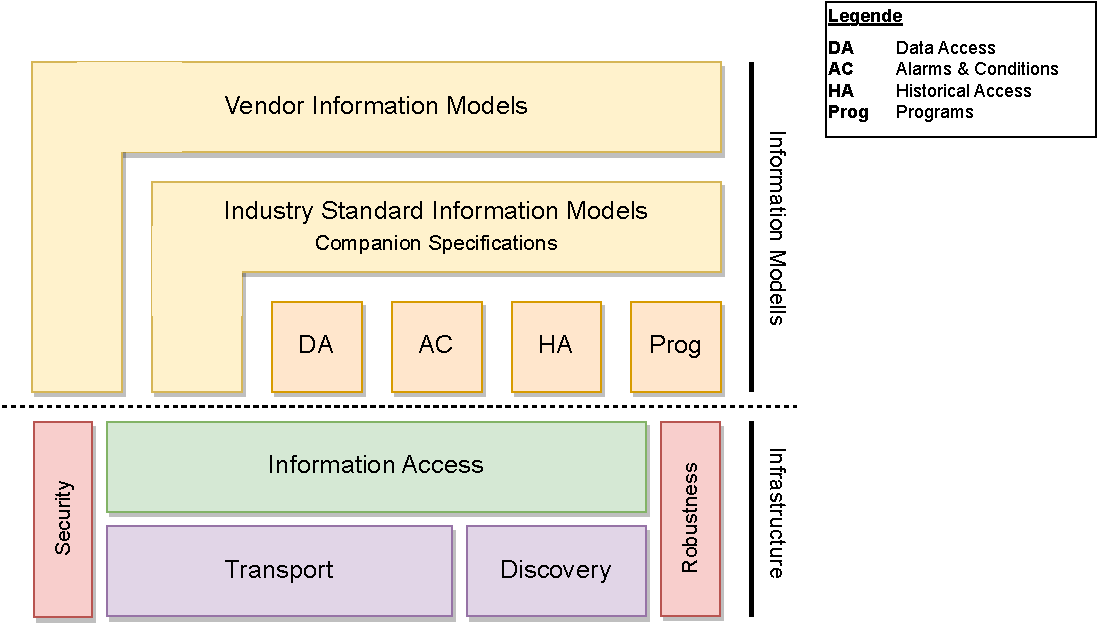
\includegraphics[width=0.9\textwidth]{res/diagramms/companionSpezifikations.pdf}
			\caption{Aufbau des OPC UA Standards, \\ Angelehnt an: Abbildung 1.7 in \cite{mahnke_opc_2009}} %TODO anständig machen
			\label{fig:OPCUA_Framework}
		\end{figure}
	
		\subsection{Kommunikationsaufbau} % Noch nicht Final: Struktur? Aufbau?
		
		OPC UA besteht aus drei Komponenten, deren Zusammenwirkung in Abbildung \ref{fig:OPCUA_Structure} abgebildet ist. Mehrere Field Connections, die die Sensorik oder SPS darstellen, mit welchen kommuniziert werden soll. Die Daten sollen zu den OPC UA Clients geleitet werden. Dies können \ac{HMI} oder MES-Systeme sein, die die Daten der Maschinen auswerten oder Steuerungsbefehle absenden möchten. OPC UA standardisiert diese Kommunikation über den OPC UA Server. Dieser setzt den OPC UA Standard um und stellt die notwendigen APIs zur Verfügung. \cite{rinke_was_2022}
		
		Der OPC UA Server implementiert die proprietären Kommunikationsprotokolle, die vom Maschinenhersteller entwickelt wurden, um mit den Anlagen und den Field Conections zu kommunizieren. Je nach Art der Daten, die die Maschine weiter gibt, werden die Daten auf dem OPC UA Server abgespeichert oder an den Client weiter gegeben. Ein OPC UA Server kann in zwei Formen entstehen. Der Hersteller kann seiner Maschine die OPC UA Standards bereits bei der Entwicklung einprogrammieren. Damit ist der Server in der Maschine integriert und die Maschine ist so von Beginn an OPC UA fähig. Sollte der Hersteller die Spezifikationen jedoch nicht implementieren, kann der Server auch zusätzlich zwischen die Maschine und den Client geschallten werden. Durch die Unabhängigkeit des Herstellers sind diese Server oft mit mehr Kommunikationsprotokollen ausgestattet, was deren Möglichkeiten, mit der Maschine zu interagieren erhöht. \cite{rinke_was_2022}
		
		Die Kommunikation mit dem Client läuft dabei 1 zu 1 ab. Allerdings kann auch ein 1 zu n Kommunikationsmodell über Publish and Subscribe implementiert werden. Um diese Funktion jedoch zu nutzen, muss der Server mit der OPC UA Pub/Sub Spezifikation erweitert werden. \cite{mielebacher_verteilte_2021}
		
		Der Client kann die Daten über die standardisierte API des OPC UA Servers abfragen. Es können Echtzeitdaten, historische Daten abgerufen werden. Außerdem gibt es eine Spezifikation, wie Alarmierungslogik umgesetzt werden soll. Dies wird anhand der Implementation auf Serverebene deutlich vereinfacht, da sie dann Hersteller unabhängig ist. \cite{rinke_was_2022}
		
		\begin{figure}[H]
			\centering
			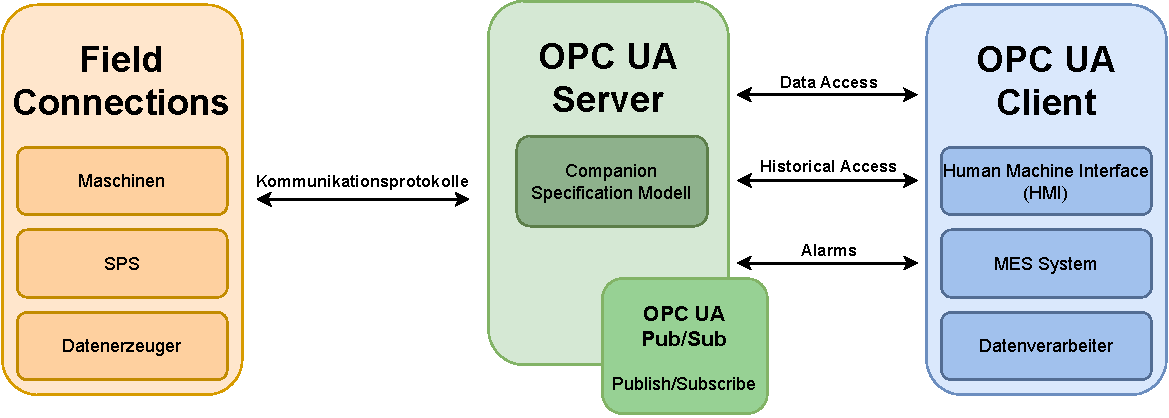
\includegraphics[width=0.9\textwidth]{res/diagramms/OPCUA.pdf}
			\caption{Kommunikationsstruktur OPC UA}
			\label{fig:OPCUA_Structure}
		\end{figure}
		
		\subsection{Sicherheit}
		
		% (0,5 bis 1 Seite)
		
		%TODO Security beschreiben
		% Wenn bei Umati sich etwas ändert, dann dort noch ein Kapitel puschen
	
	\section{Umati}
		
		
		Umati ist eine globale Initiative zur Standardisierung von Interfaces zur Kommunikation zwischen Produktionsanlagen. Sie wird vom \ac{VDMA} und dem \ac{VDW} verwaltet und vorangetrieben von den Zahlreichen Mitgliedern der beiden Vereinigungen. Das Ziel ist es die Kommunikation zwischen Maschinen möglichst einfach, sicher und einfach zu gestalten. Es soll eine Plug \& Play Umgebung entstehen in der neue Maschinen in eine Anlage durch bloßes einstecken ins Kommunikationsnetzwerk integriert werden können. Die Umati Initiative entwickelt Standards, welche weltweit zum Einsatz kommen sollen um eine startke internationale Gemeinschaft um diesen Standard zu erreichen. \cite{noauthor_umati_2023}
		
		Umati baut auf den OPC UA Standards der OPC Foundation auf. OPC UA bildet dabei die Basis und definiert wie kommuniziert werden soll und was. Es legt fest die Rahmenbedingungen für Konnektivität und syntaktische Interoperabilität. Da dieser Standard kostenfrei zur Verfügung steht, ist es die optimale Voraussetzung um weiterreichende Spezifikation auf ihn aufzubauen. \cite{noauthor_umati_2023}
		
		Umati soll vor allem die vertikale und horizontale Integration im Unternehmen erleichtern. In Abbildung \ref{fig:Automatisierungspyramide} ist die Automatisierungspyramide nach Siepmann abgebildet. Je tiefer die Pyramide nach unten geht, desto vielfältiger sind die Systeme. Während ein Unternehmen nur ein \ac{ERP} System verwendet, kann es zahlreiche SPS und noch mehr Ein- und Ausgabesensoren geben. Diese müssen vertikal Integriert werden. Dafür werden Daten von den unteren Ebenen in die Systeme weiter oben zur Verarbeitung überreicht. Bei der horizontalen Integration kommunizieren gleichartige Systeme miteinander. Beispielsweise wenn mehrere SPS Daten austauschen oder Daten Abteilungsübergreifend übergeben werden, wie bei einem Datenfluss von SCM zu CRM System sein. 
		
		\begin{figure}[H]
			\centering
			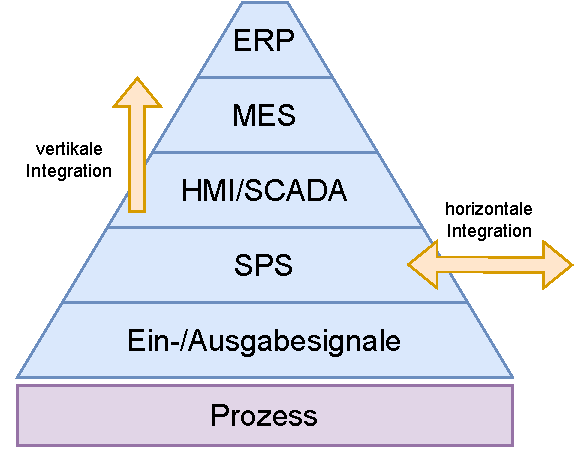
\includegraphics[width=0.8\textwidth]{res/diagramms/Automatisierungspyramide.pdf}
			\caption{Automatisierungspyramide nach Siepmann, \\ Angelehnt an: Folie 8 in \cite{mielebacher_verteilte_2021}} 
			\label{fig:Automatisierungspyramide}
		\end{figure}
		
		Umati legt standardisierte Interfaces fest, mit denen die vertikale und horizontale Integration möglichst einfach umgesetzt wird. Dadurch kann die Wertschöpfung aus Daten kostengünstiger ablaufen und die Analyse, Verarbeitung und Verwertung von Daten wie es in der Industrie 4.0 üblich ist besser ablaufen. Umati hat bereits Vorführungen auf Messen veranstaltet, welche die Funktionsfähigkeit einer Umati Umsetzung demonstrieren. Umati standardisiert dabei die Integration von Maschinen, deren Installation und ganze IT Produktionsumgebungen. \cite{noauthor_about_nodate}
	
		% Umati aufbau
		
		OPC UA hatte bereits Standards, welche in die Richtung von den Umati gehen anhand der Companion Spezifikationen definiert. Allerdings wuchs der Umfang dieser Spezifikationen über die Jahre stark an, weshalb sich Umati die Aufgabe setzt, diese Spezifikationen zu zentralisieren und somit einen gemeinsamen Standard zu erzeugen, welcher von allen Mitgliedern verwendet wird.
		
		Umati selbst besteht aus verschiedenen Modulen welche alle Standards für verschiedene Bereiche definieren. In Abbildung \ref{fig:OPCUA_for_machinery} sind alle Interfaces abgebildet, welche auf der Base Spezifikation OPC 40001 aufbauen. Dieser wird auch OPC 40001 UA for Machinery genannt und ist für die Anlagenbau Industrie gedacht. Umati befindet sich noch in der Entwicklung und ist noch nicht vollständig fertiggestellt, deshalb gibt es Interfaces, welche noch nicht umgesetzt, sondern nur geplant sind. \cite{noauthor_machinery_nodate}
		
		\begin{figure}[H]
			\centering
			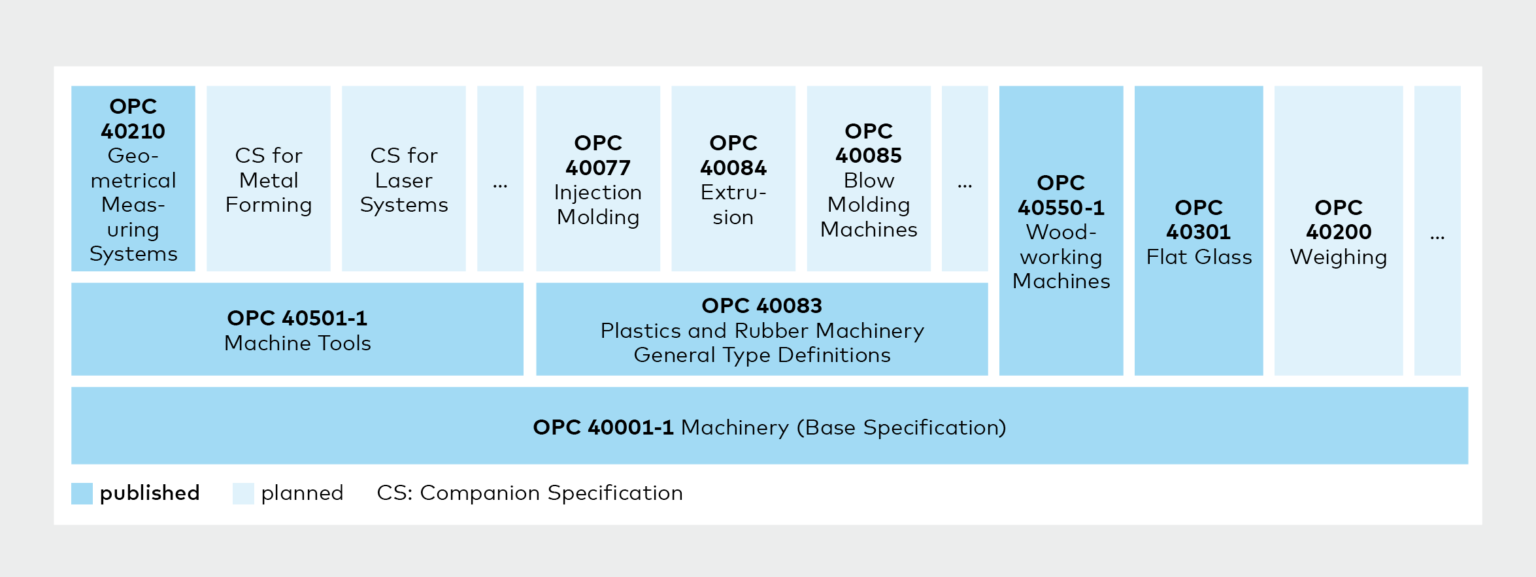
\includegraphics[width=0.9\textwidth]{res/diagramms/OPCUA_for_machinery.png}
			\caption{Interfaces basierend auf OPC UA for Machinery \cite{noauthor_machinery_nodate}} 
			\label{fig:OPCUA_for_machinery}
		\end{figure}
		
		% Kennzahlen, wer nutzt schon, was sind bisherige Meinungen dazu
		
		
	
		\subsection{VDMA}
		
		\ac{VDMA} ist der größte Industrieverbund in Europa und hat Umati ins leben gerufen hat. Der Verband wurde 1892 gegründet und hat seinen Sitz in Frankfurt am Main. Neben der Vertretung der Interessen Industrieller Unternehmen in Deutschland und Europa gegenüber der Politik, erarbeitet der VDMA auch Standards und tauscht Know-How zwischen seinen 3.600 Mitgliedsunternehmen aus. \cite{noauthor_verband_nodate} In dem Interessenverband sind Firmen aus den Bereichen Maschinenbau, Anlagenbau und der Zulieferindustrie welche sich Kompetenzen und Informationen in verschiedensten Themenbereichen von Bildung \& Modernem Arbeiten über Digitalisierung bis zu Rechtlichen Feldern teilen. \cite{noauthor_themenubersicht_nodate}
		
		Der VDMA wirkt vor allem mit Förderungen in Bereichen, die Innovation bringen. Beispielweise fördert der Verband Technologien in den Bereichen Industrie 4.0, Digitalisierung und nutzt Lobbyarbeit um seine Mitglieder auch politisch zu unterstützen. Außerdem veranstaltet der VDMA Messen zur Netzwerkbildung und zum demonstrieren von neusten Technologien seiner Mitglieder. Im allgemeinen verfolgt der Verband die Stärkung der Europäischen Maschinenbaubranche und die Verbesserung der Wettbewerbsfähigkeit auf Internationaler Ebene.
		
		AZO, der Partner dieser Arbeit, ist auch ein Mitglied des VDMA. Da AZO ein Mittelständiges Unternehmen im Anlagenbau ist, setzt sich der VDMA genau für diese Interessen ein. Umati soll eine Plug \& Play Umgebung im Anlagenbau ermöglichen. Der VDMA möchte eine erhöhte Interoperabilität zwischen den Maschinen ihrer Mitglieder bewirken und so die Wettbewerbsfähigkeit des Europäischen Markts stärken, aber auch in der Standardisierung der Internationale Industrie mitwirken. 
		
		\subsection{Anforderungen}
		
		% Was benötige ich, um Umati umzustetzen
		% Was wird benötigt zum ...
			% senden
			% empfangen
		
			% Anmeldung
		
		\subsection{OPC UA for Machinery}
		
		\texttt{OPC 40001-1/VDMA 40001-1} wurde von VDMA und VDM zusammen mit der OPC Foundation entwickelt. Es ist die Base Spezifikation auf der andere in diesem Bereich aufbauen sollen. Sie wurde im September 2020 veröffentlicht und seit dem aktualisiert worden. Der Standard wird auch in Zukunft erweitert werden um mehr Use Cases abzudecken.
		
		% OPCUA 40001 (for Machinery)
		
		% für was speziell gemacht
		% Was ist festgelegt
			


\chapter{Methodik}\label{ch:Methodiken}
	% (8 Seiten)
	
	
	% Forschungsmethodik - Deduktiv??? - Konstruktiv???
	
	\section{Literaturrecherche}
	% Datenerhebung - Literaturrecherche
	% Stichwort recherche
	
	\section{Evaluation}
	
	\section{Experteninterview}
	
	\section{Zeitplanung}
	
	\begin{figure}[H]
		\centering
		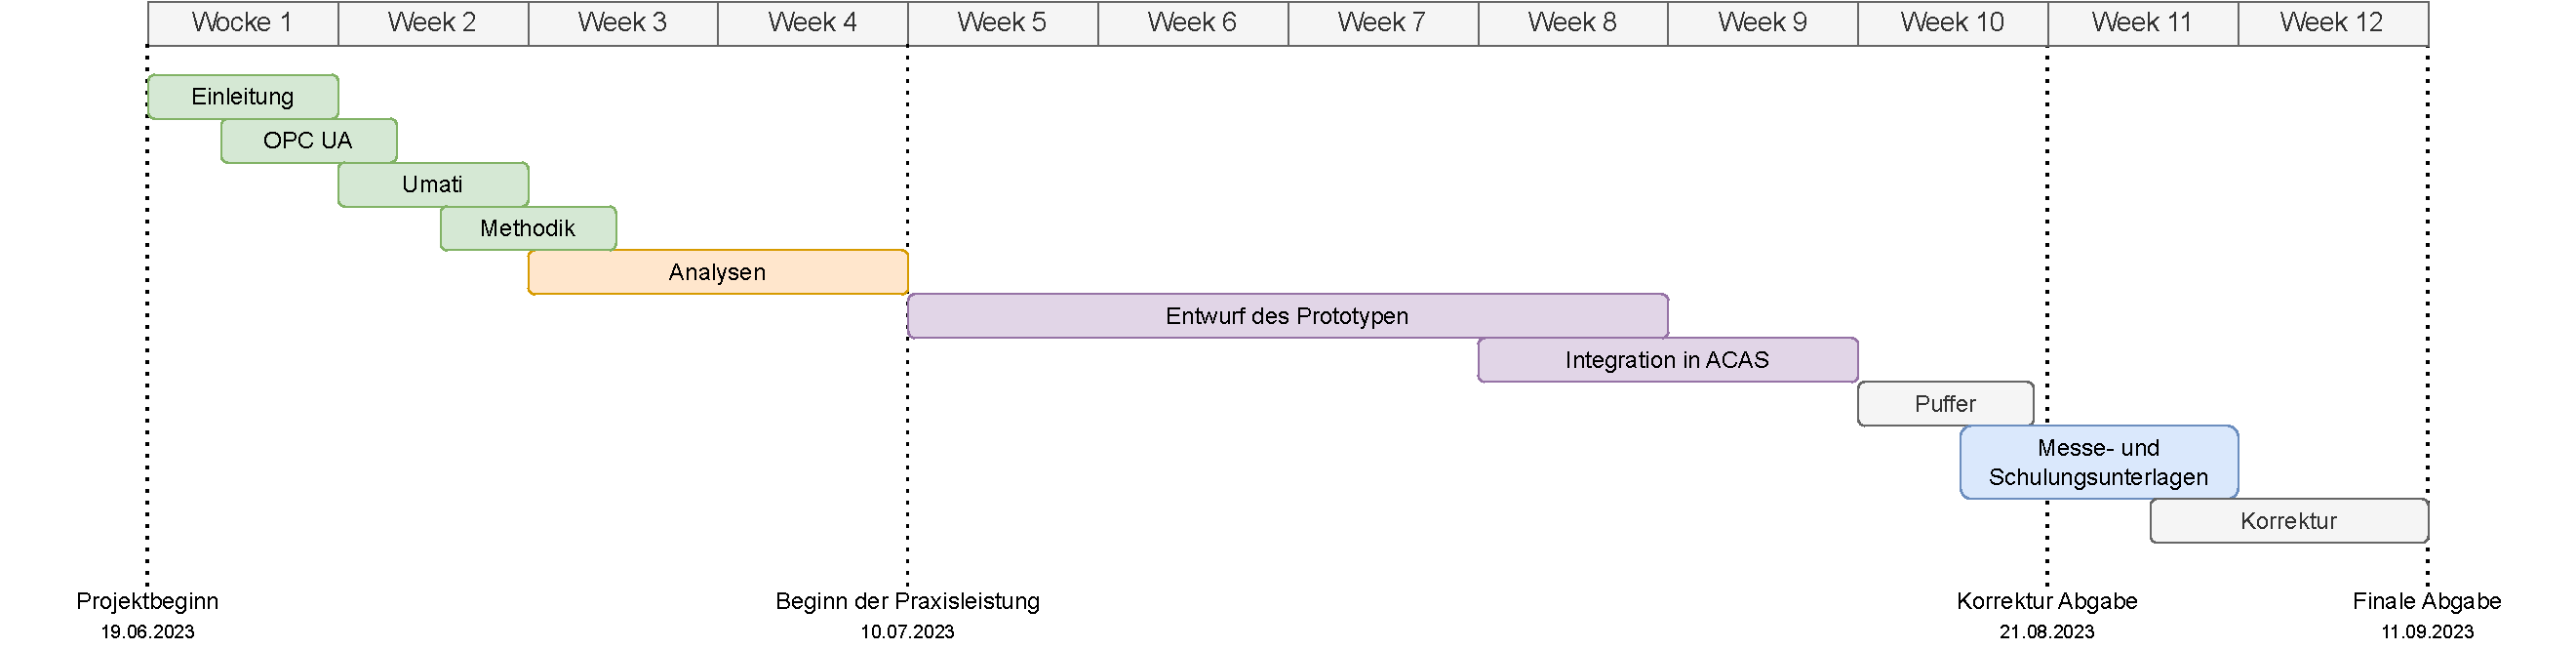
\includegraphics[width=0.9\textwidth]{res/analysen/Grantt-Diagramm.pdf}
		\caption{Grantt-Diagramm zum Projektablauf}
		\label{fig:Grantt}
	\end{figure}
	
\chapter{Ergebnisse}\label{ch:Ergebnisse}
	
	% (8 Seiten)
	
	\section{Anforderungsanalyse}
	
	\section{Lösungsansätze}
		% Nach was suche ich, Kriterienentwurf
		% Was bracuh ich Hard Soft
		
		% Literaturrecherche an anderen Implementationen (Umati und 5G)
	
	\section{Marktanalyse}
	
		% Fertige Lösungen
		% Node Red selbstimplementierung
	
	\section{Wirtschaftlichkeit und Projektanalyse}
	
		\subsection{Kostenplanung}
		
		\subsection{Fallbeispiel}
			% Beispielswiese an Fallbeispiel -> Durchschnittliche AZO Straße
			% Interview mit Person die diese Integration macht -> Expertenquellen
			% -> Probleme bei Schnittstellen integrierung.
	
	\section{Implementierung eines Prototyps}
	
		\subsection{Aufbau der Umgebung}
		
		\subsection{Implementierung}
		
			% Proof of Konzept
			% Proof of Konzept mit Node Red
			
			% Probleme und Lösungen
		
		\subsection{Integration in bestehende Infrastruktur}
			% Integration in Unternehmensstruktur
			

	
	
	\chapter{Diskussion und Fazit}\label{ch:Diskussion_Fazit}
	
		% (2-5 Seiten)	
	
		% Disskussion -> Subjektive Bewertung der Spezifikation UMATI, ... Literaturpunkte meine Meinung, Sinnvoll Einzusetzen
	
	
	\frontmatter
	\printbibliography

\end{document}
